\documentclass[article]{jss}
\usepackage[utf8]{inputenc}

\usepackage{amsmath, amsfonts, amssymb, amsthm, graphicx}
\usepackage[ruled]{algorithm2e}
\usepackage{caption}
\usepackage{tikz}

\setlength{\parindent}{0pt}
\newcommand{\forceindent}{\leavevmode{\parindent=1em\indent}}
\numberwithin{equation}{section}

\newtheorem*{theorem*}{Theorem}
\newtheorem*{cor*}{Corollary}

\newcommand{\norm}[1]{\left\lVert#1\right\rVert}
\newcommand{\e}{\epsilon}
\newcommand{\w}{\omega}
\newcommand{\R}{\mathbb{R}}
\newcommand{\N}{\mathbb{N}}
\newcommand{\Q}{\mathbb{Q}}
\newcommand{\Z}{\mathbb{Z}}
\renewcommand{\ae}[1]{\text{ \hspace{5pt} a.e. #1}}


\author{Austin David Brown\\University of Minnesota}

\title{Combining $l^1$ and Higher Order $l^p$ Penalization in Regression Models}

\Abstract{
We create the package Penalized Regression on Steroids (\textbf{pros}) to combine $l^1$ penalized regression with higher order $l^p$ penalizations built upon the elastic-net idea. The package is able to fit regression models with penalizations ranging from $l^1$ to $l^{10}$.
}

\Keywords{Penalized Regression, \proglang{C++}, \proglang{Python}, \proglang{R}}
\Plainkeywords{Penalized Regression, C++, R, Python}

\Address{
  Austin David Brown \\
  University of Minnesota \\
  Department of Statistics (Graduate Student) \\
  E-mail: \email{Brow5079@umn.edu}
}

\begin{document}

\section{Introduction}

In statistics and probability theory it is common to impose moment assumptions on a random variable $X : \Omega \to \R^n$ such as $E(|X|^k) < \infty$ for $k \in \N$.
These constraints correspond to the $L^p$ spaces which allow control over the width and the height of such random variables.
Constraints of this type may also be motivated geometrically.
Consider for example an elastic-net penalty $Q(x) = \frac{1}{2} |x| + \frac{1}{2} |y| + \frac{1}{2} |x|^2 + \frac{1}{2} |y|^2 \le 1$
shown on the left and a new penalty $P(x) = \frac{1}{2} |x| + \frac{1}{2} |y| + \frac{1}{2} |x|^4 + \frac{1}{2} |y|^4 \le 1$ shown on the right.

\begin{minipage}{.5\textwidth}
  \centering
  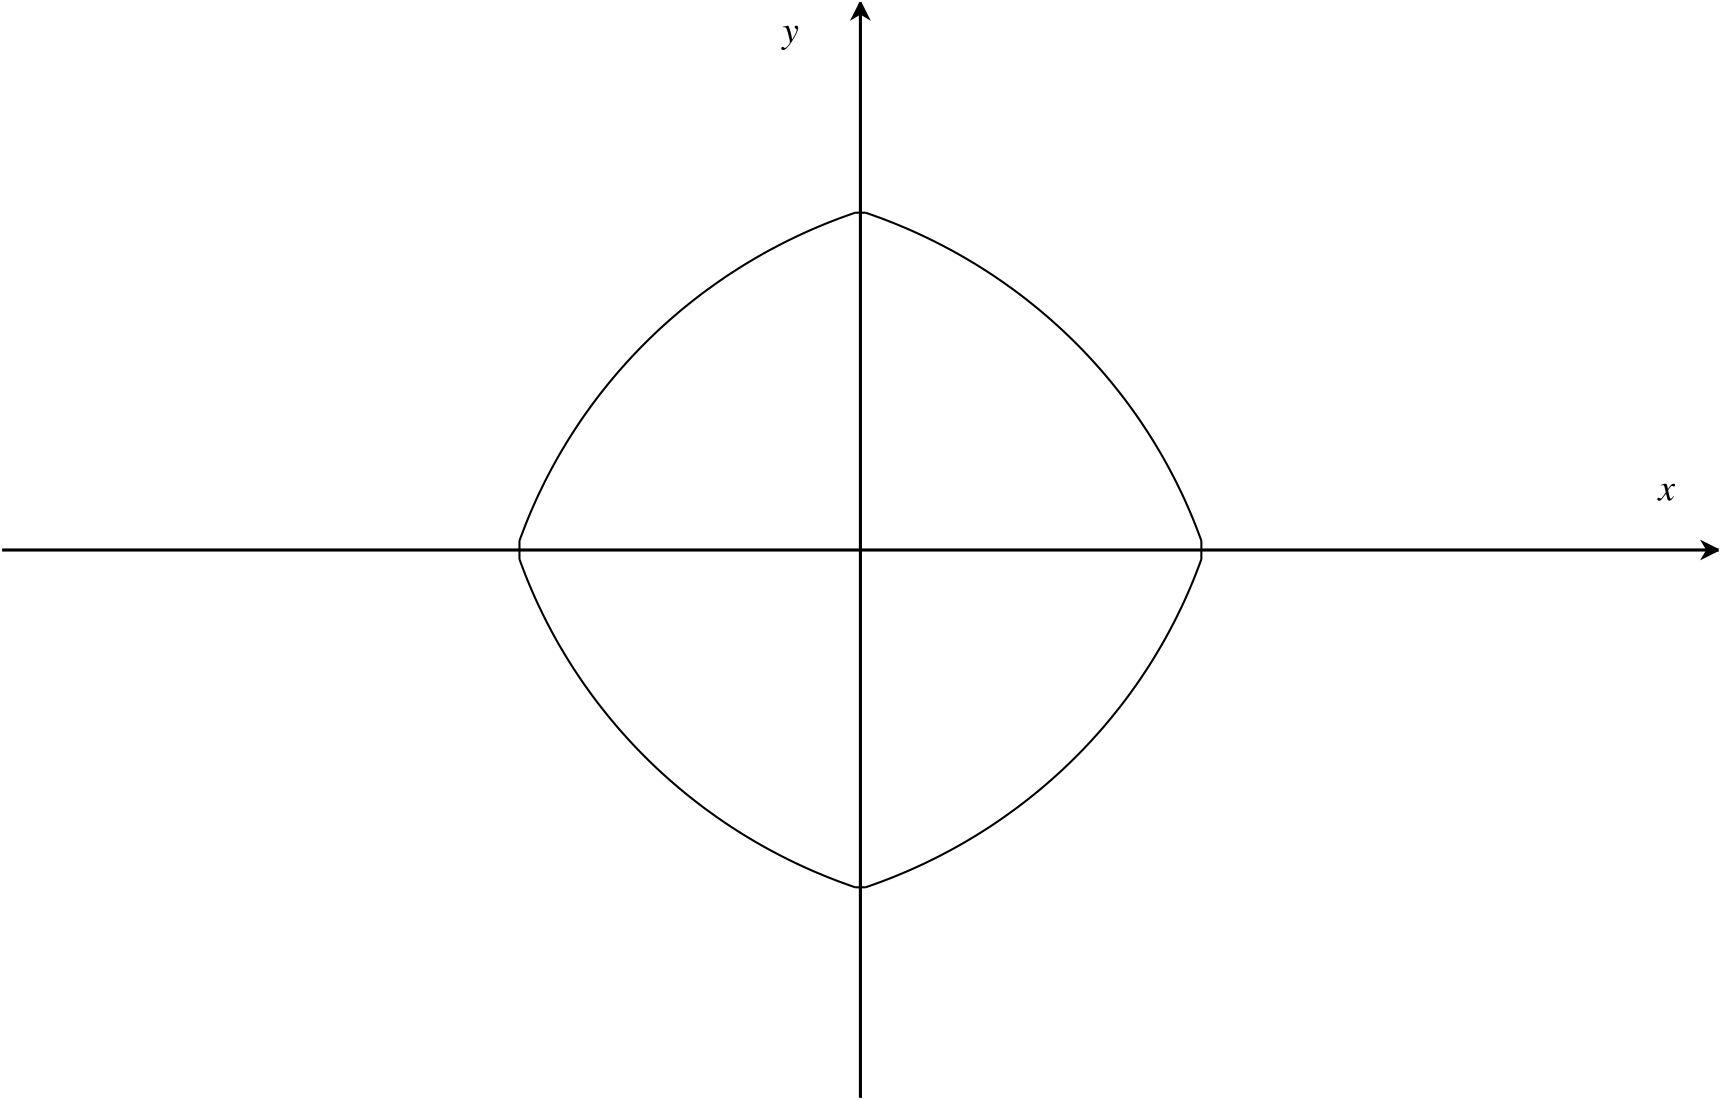
\includegraphics[width=.8\linewidth]{elasticnet.png}
\end{minipage}%
\begin{minipage}{.5\textwidth}
  \centering
  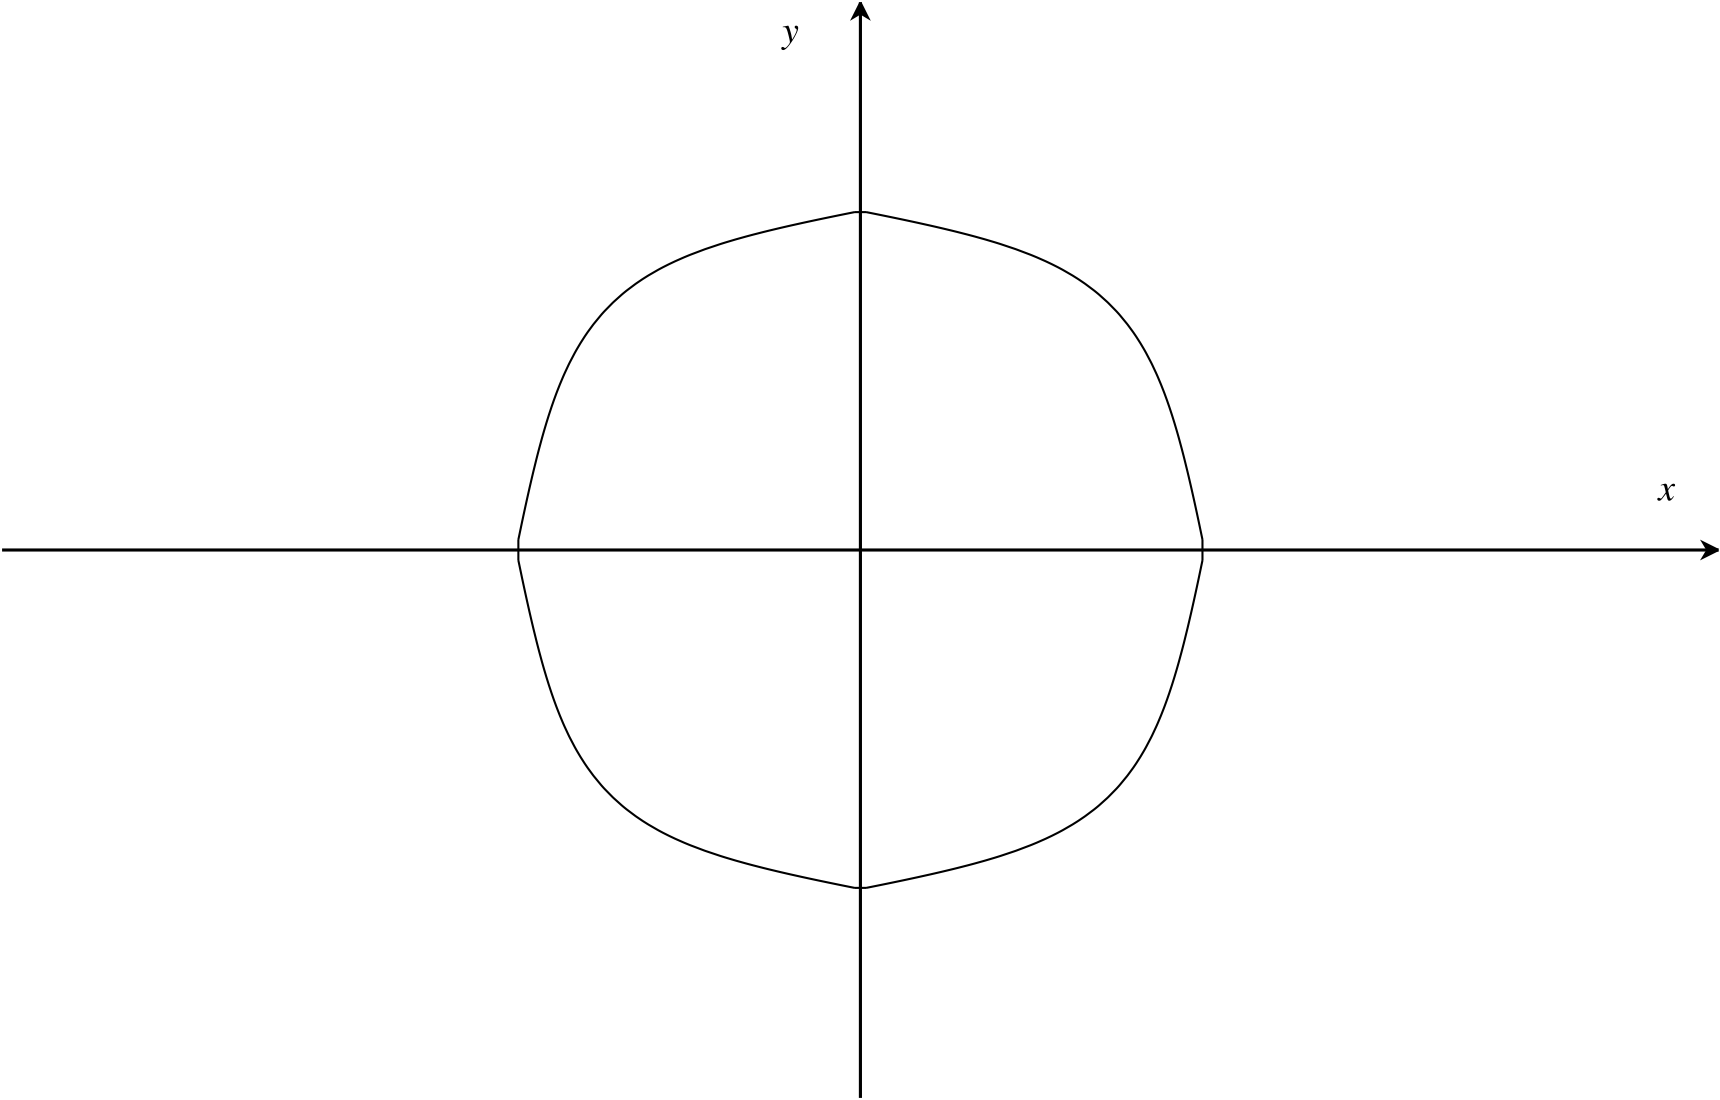
\includegraphics[width=.8\linewidth]{new_penalty_4_moment.png}
\end{minipage}
\captionof{figure}{A particular elastic-net penalty shown on the left and a new penalty shown on the right shown to "bow" out the penalization while retaining convexity.}

It seems reasonable that a scientist may want more control over the height and width of the penalization while still retaining sparse solutions in regression models.
In this project, we build the Penalized Regression on Steroids (\textbf{pros}) package to expand upon the idea of the elastic-net by \cite{elasticnet}, which we believe approximately encapsulates this idea.

\section{Penalized Regression Implementation}

In this section, we discuss how the \textbf{pros} package was implemented. In particular, the construction of the problem and the algorithms used.
First, we formulate the regression model with a new penalization.
Let
\[
L_{\lambda}(\beta) = \frac{1}{2} \norm{y - \beta_0 1 - X \beta}_2^2 + \lambda P(\beta)
\]
be the objective to minimize with penalty
\[
\lambda P(\beta) = \lambda \alpha_0 \norm{\beta}_1 + \lambda \sum_{k = 1}^{5} \alpha_k \norm{\beta}_{2k}^{2k} 
\]
where $y \in \R^n$, $X \in M_{n \times p}(\R)$, and $(\beta_0, \beta) \in \R^p$, $\lambda \in \R_{+}$ and $\alpha$'s are convex combinations.
This penalty is convex and completely separable which allows for coordinate-wise optimization.
The coordinate descent algorithm is very successful for the elastic-net penalty due to the \textbf{glmnet} package by \cite{glmnet}.
Further, with the elastic-net penalty, the coordinate wise minimization yields an analytic, closed form solution at each iteration avoiding any need for a line search or step size.
The penalty that we propose lacks an analytic solution and thus a new algorithm is needed.

\subsection{Optimization Algorithms and Implementation}

The first algorithm utilized was the subgradient coordinate algorithm shown below.

\vspace{.2cm}
\begin{algorithm}[H]
\caption{Subgradient Coordinate Algorithm}
Choose $\beta^0 \in \R^p$, tolerance $\delta > 0$, $R > 0$, and maximum iterations $N$.

Set $k \gets 0$

Set the step size $h \gets \frac{R}{\sqrt{1 + N}}$

\Repeat{Until the objective difference is less than $\delta$}{ 

  Permute $I = \{1, \ldots, p\}$

  \For {$i \in I$}{

    $\beta^{k + 1}_i \gets \beta^{k}_i - h g^i$ where $g^k_i \in (\partial L_\lambda(\beta^k))_i$

    $k \gets k + 1$
  }
}

\end{algorithm}
\vspace{.2cm}

The drawbacks of this algorithm include lack of the descent property, no good stopping criterion, and many possible choices for the subgradient.
The step size is optimal and chosen due to \cite{nesterov} with a worst case convergence rate of $O(\frac{1}{\sqrt{k}})$.
Ultimately, no line search can be implemented and the step size must be tuned by the user, which may be difficult for inexperienced users.
Another drawback is that this particular stopping criterion is expensive at $O(n^2)$ flops at each iteration.

Due to the separability of the penalization, a better algorithm is proximal gradient coordinate descent shown below.

\vspace{.2cm}
\begin{algorithm}[H]
\caption{Proximal Gradient Coordinate Descent}
Choose $\beta^0 \in \R^p$ and tolerance $\delta > 0$;

Set $k \gets 0$

\Repeat{Until the Moreau-Yoshida mapping $M_{h_k, f} < \delta$}{ 


  Randomly permute $I = \{1, \ldots, p\}$

  \For {$i \in I$}{
    Set the step size $h_i > 0$ or use line search.

    $\beta^{k + 1}_i \gets (\textbf{prox}_{h_i L})_i ( \beta^k_i - h^k \langle X_i, y - X \beta \rangle )$

    $k \gets k + 1$
  }

}
\end{algorithm}
\vspace{.2cm}

A major benefit of this algorithm is that it recovers the worst case convergence of $O(\frac{1}{k})$ even though the objective is not differentiable. The convergence analysis of coordinate descent algorithms is explored by \cite{nesterov2}. The stopping criterion chosen here is cheap to compute at $O(p)$ flops. Finally, since this is a descent method, line search may be implemented, which potentially makes the algorithm easier to use by inexperienced users.

\subsection{Cross-Validation Algorithms and Implementation}

In order to tune the Lagrangian dual variable $\lambda$, K-fold cross validation is implemented.
To improve the speed of cross-validation, a warm start algorithm is used defined below.

\vspace{.2cm}
\begin{algorithm}[H]
\caption{Warm Start Cross-Validation}
Choose a sequence of Langrangian dual variables $\lambda_1, \ldots, \lambda_N$, and initial value $\beta^0$.

Order $\lambda_{(1)}, \ldots, \lambda_{(N)}$ descending.

$\beta^{Warm} \gets \beta^0$ 

\For{$k \in 1, \ldots, N$}{

  $\beta^k \gets$ by Cross-Validation with $\lambda_{(k)}$ warm started with $\beta^{Warm}$.

  $\beta^{Warm} \gets \beta^k$
}

\end{algorithm}
\vspace{.2cm}

A difficult problem in general is choosing the sequence of $\lambda$'s.
In \textbf{glmnet}, the default is to choose a sequence of length $100$ starting from the first $\lambda_{max}$ where $\beta$ is completely zero to the lower value $.001 \lambda_{max}$ on a log-scale.
The lower $\lambda$ value in the sequence is a real difficulty and this implementation does not fully address this.
Due to time, we implement a similar but cruder default choice.
We choose the lower $\lambda_{min} = cp$ where $p$ number of columns in the predictor matrix $X$ and $c$ is chosen to be $\frac{3}{2}$. We then create a sequence of length $100$ from this lower value.
A comparison of the default choices is explored in a subsequent section.

\subsection{Step Size Rules and Line Search Implementation}

The lack of an analytic solution introduces a necessary step size rule in order to fit a regression model with the new penalization.
A good line search method due to \cite{beck_teboulle} requires an evaluation of the objective function over the entire dataset at each iteration. This has a computational complexity of $O(n^3)$ flops at each iteration. This was attempted, but never fully implemented for this reason. Instead, a user defined step size rule is required. Thus, poor step size choices do not guarantee convergence.
This is a suboptimal choice, but allows the potential for the package to be applied to large datasets.

We introduce a possible alternative algorithm to address the issue.

\vspace{.2cm}
\begin{algorithm}[H]
\caption{Step Size Tuning Avoidance Algorithm}
Choose initial value $\beta^0$, initial step size $h$, and maximum iterations $N$.

\Repeat{Until Proximal Gradient Coordinate Descent convergences}{
$h \gets \frac{1}{2}h$

$\beta \gets$ by Proximal Gradient Coordinate Descent with step size $h$
}

\end{algorithm}
\vspace{.2cm}

If the maximum iterations are not too large, this may allow users to avoid having to tune a step size while retaining good performance. We can also modify this algorithm to be run in parallel. Currently, this is not implemented due to time constraints for the project.

\section{The Penalized Regression on Steroids Package}

\subsection{Package Architecture}

The package \textbf{pros} is built using C++ and the Eigen library by \cite{eigen} is utilized for fast matrix computations. This is analogous to using Fortran with LAPACK by \cite{lapack}.
The \textbf{pros} library is not dependent on R.
To interact with R, 2 interfacing layers are needed: an R to C interface and an R program defining user callable functions.
The benefit is that many other popular programming languages can be interfaced easily.
The following diagram illustrates this idea showing that the \textbf{pros} package is more general than just an R package.

\vspace{.5cm}
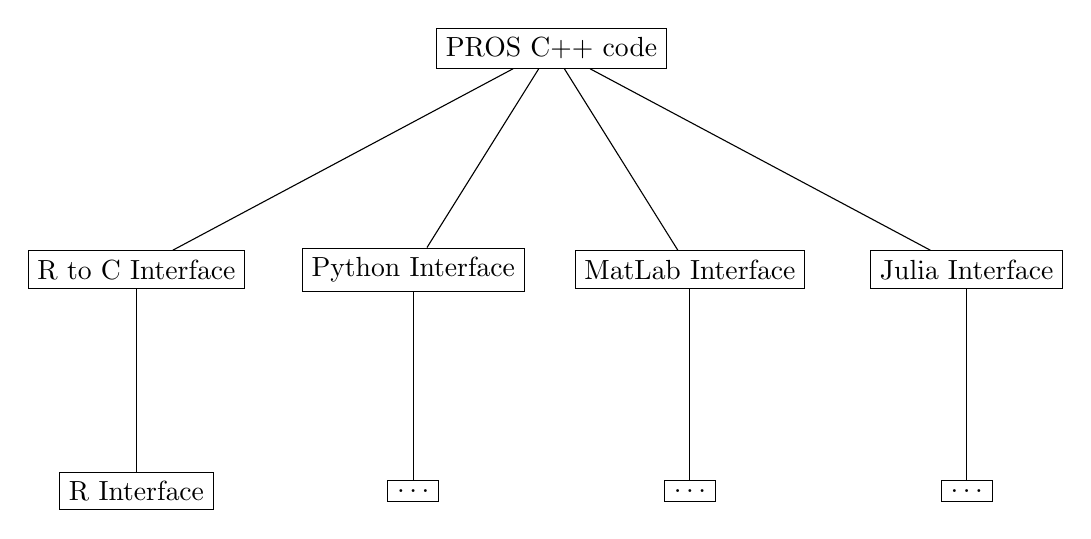
\begin{tikzpicture}[level distance=8em, sibling distance=10em,
  every node/.style = {shape=rectangle, draw, align=center}]]
  \node {PROS C++ code}
    child { node {R to C Interface} 
      child { node {R Interface} }
    }
    child { node {Python Interface} 
      child { node {$\ldots$} }
    }
    child { node {MatLab Interface} 
      child { node {$\ldots$} }
    }
    child { node {Julia Interface} 
      child { node {$\ldots$} }
    };
\end{tikzpicture}
\captionof{figure}{Illustrates interfacing the \textbf{pros} package with other languages.}
\vspace{.5cm}


The R interface in its simplest form is comprised of 2 functions.
A single fitting function with prediction

\begin{verbatim}
> fit <- pros(X, y, alpha)
> predict(fit, X)
\end{verbatim}

and a cross-validation function with prediction

\begin{verbatim}
> cv <- cv.pros(X, y, alpha)
> predict(cv, X)
\end{verbatim}

We illustrate the usage of these functions in the following sections.

\subsection{The Regression Fitting Function}

The \textbf{pros} function is used to fit a single regression model with a specified $\lambda$ for penalization. The signature of this function at the time of this paper is as follows:

\begin{itemize}
\item \code{X} is an $n \times m$-dimensional matrix of the data.

\item \code{y} is an $n$-dimensional vector of response values.

\item \code{alpha} is a $6$-dimensional vector of the convex combination corresponding to the penalization:
 \begin{itemize}
   \item $\alpha_1$ is the $l^1$ penalty.
   \item $\alpha_2$ is the $l^2$ penalty.
   \item $\alpha_3$ is the $l^4$ penalty.
   \item $\alpha_4$ is the $l^6$ penalty.
   \item $\alpha_5$ is the $l^8$ penalty.
   \item $\alpha_6$ is the $l^{10}$ penalty.
\end{itemize}

\item \code{lambda} is the Lagrangian dual penalization parameter.

\item \code{step\_size} is a tuning parameter defining the step size. Larger values are more aggressive and smaller values are less aggressive.

\item \code{algorithm} is the optimization algorithm
\begin{itemize}
\item \code{proximal_gradient_cd} uses proximal gradient coordinate descent.
\item \code{subgradient_cd} uses subgradient coordinate descent.
\end{itemize}

\item \code{max\_iter} is the maximum iterations the algorithm will run regardless of convergence.

\item \code{tolerance} is the accuracy of the stopping criterion.

\item \code{random seed} is the random seed used in the algorithms.

\end{itemize}

\subsection{The Cross-Validation Function}

The \textbf{cv.pros} function is used for K-fold cross-validation.
The warm-start algorithm and default choices for the $\lambda$ sequence are implemented as described in the previous section.
The arguments of this function are similar to the \textbf{pros} function:

\begin{itemize}
\item \code{X} is an $n \times m$-dimensional matrix of the data.

\item \code{y} is an $n$-dimensional vector of response values.

\item \code{alpha} is a $6$-dimensional vector of the convex combination corresponding to the penalization:
 \begin{itemize}
   \item $\alpha_1$ is the $l^1$ penalty.
   \item $\alpha_2$ is the $l^2$ penalty.
   \item $\alpha_3$ is the $l^4$ penalty.
   \item $\alpha_4$ is the $l^6$ penalty.
   \item $\alpha_5$ is the $l^8$ penalty.
   \item $\alpha_6$ is the $l^{10}$ penalty.
\end{itemize}

\item \code{K\_fold} is the number of folds in cross-validation.

\item \code{lambdas} is a vector of dual penalization values to be evaluated.

\item \code{step\_size} is a tuning parameter defining the step size. Larger values are more aggressive and smaller values are less aggressive.

\item \code{algorithm} is the optimization algorithm
\begin{itemize}
\item \code{proximal_gradient_cd} uses proximal gradient coordinate descent.
\item \code{subgradient_cd} uses subgradient coordinate descent.
\end{itemize}

\item \code{max\_iter} is the maximum iterations the algorithm will run regardless of convergence.

\item \code{tolerance} is the accuracy of the stopping criterion.

\item \code{random seed} is the random seed used in the algorithms.

\end{itemize}

\subsection{Possible CRAN Submission}

At the time of this paper, the \textbf{pros} package could potentially be submitted to the Comprehensive R Archive Network (CRAN).
According to the R check, there are no warnings.
However, one issue with CRAN is that in order for the user to get high performance, they will need to update their own Makevars file. The instructions for this are outlined in the \textbf{pros} repository.

\section{Numerical Examples}

\subsection{The Analysis Procedure}

The analysis for the subsequent experiments is performed in the following way:

\begin{itemize}

\item The data is split into a training and test set.

\item The predictor data are standardized.

\item The \textbf{glmnet} library and the \textbf{pros} library are used for fitting. The \textbf{glmnet} library provides varying results for a single seed so a range of values are reported.

\item 10-fold cross-validation is used to tune the Lagrangian dual variable $\lambda$.

\item The metric for comparison is the \textit{test mean squared error} defined as
\[
\frac{1}{n}\sum_{k = 1}^n \left( y_i - \hat \beta_0 1 - X_i^T \hat \beta \right)^2
\]

where $\hat \beta_0, \hat \beta$ are fit over the training set and $y$ and $X$ are the response and predictor matrix belonging to the test set.

\item The source code for this analysis is openly available at the \textbf{pros} repository available here \cite{pros}.

\end{itemize}

\subsection{The Boston Housing Dataset}

The Boston Housing dataset is popular from \cite{boston_housing}.
There are 13 predictors and the response is the median value of owner-occupied homes in \$1000's. 
The data is randomly split into a training set with 404 observations and a test set with 102 observations.
We compare default implementations between the two libraries:

\begin{center}
\setlength{\tabcolsep}{20pt} % Default value: 6pt
\renewcommand{\arraystretch}{1} % Default value: 1
\begin{tabular}{lllp{7.4cm}}
\hline
Penalty & Tuning & Test Mean Squared Error \\ \hline
Lasso (glmnet) & $\alpha = 1$ & 26.96866-28.45781 \\
elastic-net (glmnet) & $\alpha = 1/2$  & 26.55704-26.86488   \\
Lasso (pros) & $\alpha = 1$ &  26.47315 \\
elastic-net (pros) & $\alpha = 1/2$ &  26.07919 \\
$l^1$ and $l^{4}$ (pros) & $\alpha = 1/2$ &  25.5008 \\
$l^1$ and $l^{10}$ (pros) & $\alpha = 1/2$ &  30.54759 \\ \hline
\end{tabular}
\end{center}

Next, we compare manually tuned results using \textbf{pros}:

\begin{center}
\setlength{\tabcolsep}{20pt} % Default value: 6pt
\renewcommand{\arraystretch}{1} % Default value: 1
\begin{tabular}{lllp{7.4cm}}
\hline
Penalty & Tuning & Test Mean Squared Error \\ \hline
elastic-net (pros) & $\alpha = 0.1$ & 25.52578 \\
$l^1$ and $l^{4}$ (pros) & $\alpha = 0.6$ &  25.44149 \\
$l^1$ and $l^{10}$ (pros) & $\alpha = 0.9$ &  25.68279 \\ \hline
\end{tabular}
\end{center}

The three different penalizations each select all of the variables and provide no sparsity in the manually tuned scenario.

\subsection{The Prostate Dataset Analysis}

This is a popular dataset from \cite{prostate}.
There are 8 predictors and the response is the log of the prostate specific antigen.
We compare default implementations between the two libraries:

\begin{center}
\setlength{\tabcolsep}{20pt} % Default value: 6pt
\renewcommand{\arraystretch}{1} % Default value: 1
\begin{tabular}{lllp{7.4cm}}
\hline
Penalty & Tuning & Test Mean Squared Error \\ \hline
Lasso (glmnet) & $\alpha = 1$ & 0.4443432-0.4646501 \\
elastic-net (glmnet) & $\alpha = 1/2$  & 0.4539684-0.4633808   \\
Lasso (pros) & $\alpha = 1$ &  0.4457657 \\
elastic-net (pros) & $\alpha = 1/2$ &  0.4637193 \\
$l^1$ and $l^{4}$ (pros) & $\alpha = 1/2$ &  0.4621351 \\ \hline
\end{tabular}
\end{center}

Next, we compare manually tuned results using \textbf{pros}:

\begin{center}
\setlength{\tabcolsep}{20pt} % Default value: 6pt
\renewcommand{\arraystretch}{1} % Default value: 1
\begin{tabular}{lllp{7.4cm}}
\hline
Penalty & Tuning & Test Mean Squared Error \\ \hline
elastic-net (pros) & $\alpha = .99$ & 0.4441737 \\
$l^1$ and $l^{4}$ (pros) & $\alpha = .99$ &  0.4441405 \\
$l^1$ and $l^{10}$ (pros) & $\alpha = .99$ &  0.4441301 \\ \hline
\end{tabular}
\end{center}

In the manually tuned case, all three penalizations select the same variables $(\beta_1, \beta_2, \beta_4, \beta_5, \beta_8)$, which is not the optimal choice according to \cite{elasticnet}. Interestingly, all of the best values share the same $\lambda$ value.

\subsection{Conclusion}

It appears the new penalty can sometimes produce a minor improvement over the elastic-net penalty.
However, there was much to learn in the implementation.
Creating an R package is much more difficult than anticipated and CRAN is stringent on the requirements.
Comparing against other packages can also be difficult.
One source of confusion was noticing that \textbf{glmnet} uses a transformation for their $\lambda$ values and these do not correspond with the typical Lasso model formulation. Thus, direct comparisons are complicated. Further adding to the complication is that \textbf{glmnet} provides varying results for fixed random seeds.
More time should have been spent carefully reviewing the \textbf{glmnet} paper by \cite{glmnet}. Due to this, the values in the corresponding slides for this project are incorrect. 


\bibliography{project}

\end{document}

